%!TEX root = ../../Main.tex
\graphicspath{{Chapters/Mikrofonmontering/}}
%-------------------------------------------------------------------------------

\chapter{Transport::send}

Meningen med vores Transport::send er, at lave forskellige "sikkerheds tjek" på vores buffer[], altså den data vi ønsker at sende til clienten. De "sikkerheds tjek" vi laver på vores data, består af den Header man kan se på billedet nedenfor:\\
\begin{figure}[H]
	\centering
	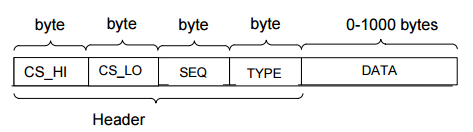
\includegraphics[width = 300 pt]{Img/header.PNG}
	\caption{Header tansportlag}
	\label{fig:konceptbillede}
\end{figure}

Headerens to byte med checksum-beregning, er henholdsvis mest betydende og mindst betydende del af chechsum beregningen. Der bliver også tildelt et sekvensnummer på det afsendte segment. Den sidste del af headeren er TYPE, som afgører alt efter om det er et 1 eller et 0 om det er et ark, eller data der bliver sendt med.\\
Meningen med at denne header bliver lagt til dataen i transportlaget, er så når data-pakken når clienten og funktiot. 
nen Transport::receive() bliver kørt. Så kan data i pakken tjekkes for checksum, sekvensnummer samt kontrollere om ark beskeder sendt rigtig.\\
I koden for vores Transport::send, som ses nedenfor, starter vi med at lægge alt fra buf[] over i buffer. Efter vi har lagt det over i buffer bruger vi funktionen calcChecksum(), som fylder pladserne CS HI og CS LO i headeren som ses på billedet ovenfor. \\
Nedenunder dette ligger der en if-løkke der sørger for at, hvis data'en bliver ødelagt, at pakken bliver sendt påny.


\begin{lstlisting}[frame=single]  % Start your code-block

void Transport::send(const char buf[], short sizeApp)
{
int i;

do{
i = 0;
buffer[TYPE] = DATA;
buffer[SEQNO] = seqNo;

for(i = 0; i < sizeApp; i++)    //Laegger buf over i buffer
{
buffer[i+ACKSIZE] = buf[i];
}

checksum->calcChecksum(buffer, sizeApp+ACKSIZE);


if(CORRUPT_DATA == 1)
{
buffer[0] = 0;
std::cout << "Bit oedelagt" << std::endl;
}
link->send(buffer, i+ACKSIZE);




CORRUPT_DATA++;

} while(!receiveAck());

}
}
\end{lstlisting}

